\documentclass[border=1pt]{standalone}

\usepackage{tikz}
\usetikzlibrary{angles,calc,intersections,quotes,arrows.meta}

\begin{document}

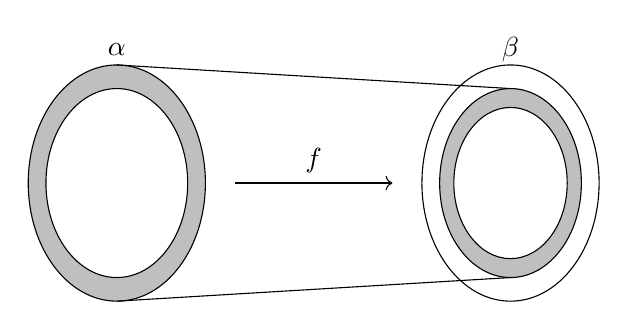
\begin{tikzpicture}
\draw (0, 1.7) node {$\alpha$};
\draw[fill=gray!50] (0, 0) ellipse (1.125 and 1.5);
\draw[fill=white] (0, 0) ellipse (1.125*0.8 and 1.5*0.8);

\draw (5, 1.7) node {$\beta$};
\draw (5, 0) ellipse (1.125 and 1.5);
\draw[fill=gray!50] (5, 0) ellipse (1.125*0.8 and 1.5*0.8);
\draw[fill=white] (5, 0) ellipse (1.125*0.64 and 1.5*0.64);

\draw (0, 1.5) -- (5, 1.5*0.8);
%\draw (0, 1.5*0.8) -- (5, 1.5*0.64);
\draw (0, -1.5) -- (5, -1.5*0.8);
%\draw (0, -1.5*0.8) -- (5, -1.5*0.64);

\draw [->] (1.5, 0) -- (3.5, 0) node [pos=0.5, above] {$f$};

\end{tikzpicture}

\end{document}
